\begin{fullwidth}
    \section{The dYdX Chain Migration} \label{sec:migration}

    \begin{adjustwidth}{2cm}{2cm}
        \justify
        dYdX's migration from Ethereum to dYdX Chain involves several moving parts, the most crucial of which was choosing dYdX Chain's L1 staking token. In a recent governance proposal made by Wintermute governance, voters elected DYDX as the chain's L1 token, a natural choice. A key challenge then arises: bridging ethDYDX from Ethereum to dYdX Chain. In this section, we provide a chronology of this migration process. Throughout this section we will refer to Ethereum-based DYDX as ethDYDX, and dYdX Chain DYDX as DYDX.
    \end{adjustwidth}
    
    \textcolor{gray}{\rule{\linewidth}{0.1mm}}
    
\end{fullwidth}

    The dYdX Foundation launched the ethDYDX token in August 2021. From inception, the ethDYDX token was owned and controlled by dYdX token holders (collectively, the ``community'', ``governance'', or the DAO). Token holders can exercise this control in several ways: they may increase or decrease the distribution of rewards, transact ethDYDX from the community's treasury, and upgrade a number of smart contracts pertaining to the ethDYDX token. Token holders vote on what actions to take through the governance process. 

    The migration of the dYdX ecosystem was largely a question of whether or not to migrate the ethDYDX token from Ethereum to dYdX Chain and make it the chain's staking token. On September 1st, 2023 the community voted in favor of setting DYDX as dYdX Chain's staking token, and ratified a wrapped version of ethDYDX, wethDYDX, to serve as a new governance token for dYdX v3 on Ethereum. For the remainder of this section, we discuss the steps involved with bridging ethDYDX and other community resources to dYdX Chain, as well as other actions the community has taken, or might take in the future to ensure a successful launch for dYdX v4.

    \subsection{Adopting the dYdX v4 Software}

        The first major step in migrating the dYdX ecosystem was adopting the open-source software built by dYdX Trading as the de facto next iteration of the dYdX exchange. Wintermute governance submitted a \bhref{https://dydx.forum/t/drc-v4-adoption-dydx-token-migration-to-dydx-chain/970}{governance proposal}, ratifying this adoption of the v4 software in a snapshot vote in August, 2023.

        \begin{marginfigure}
            \centering
            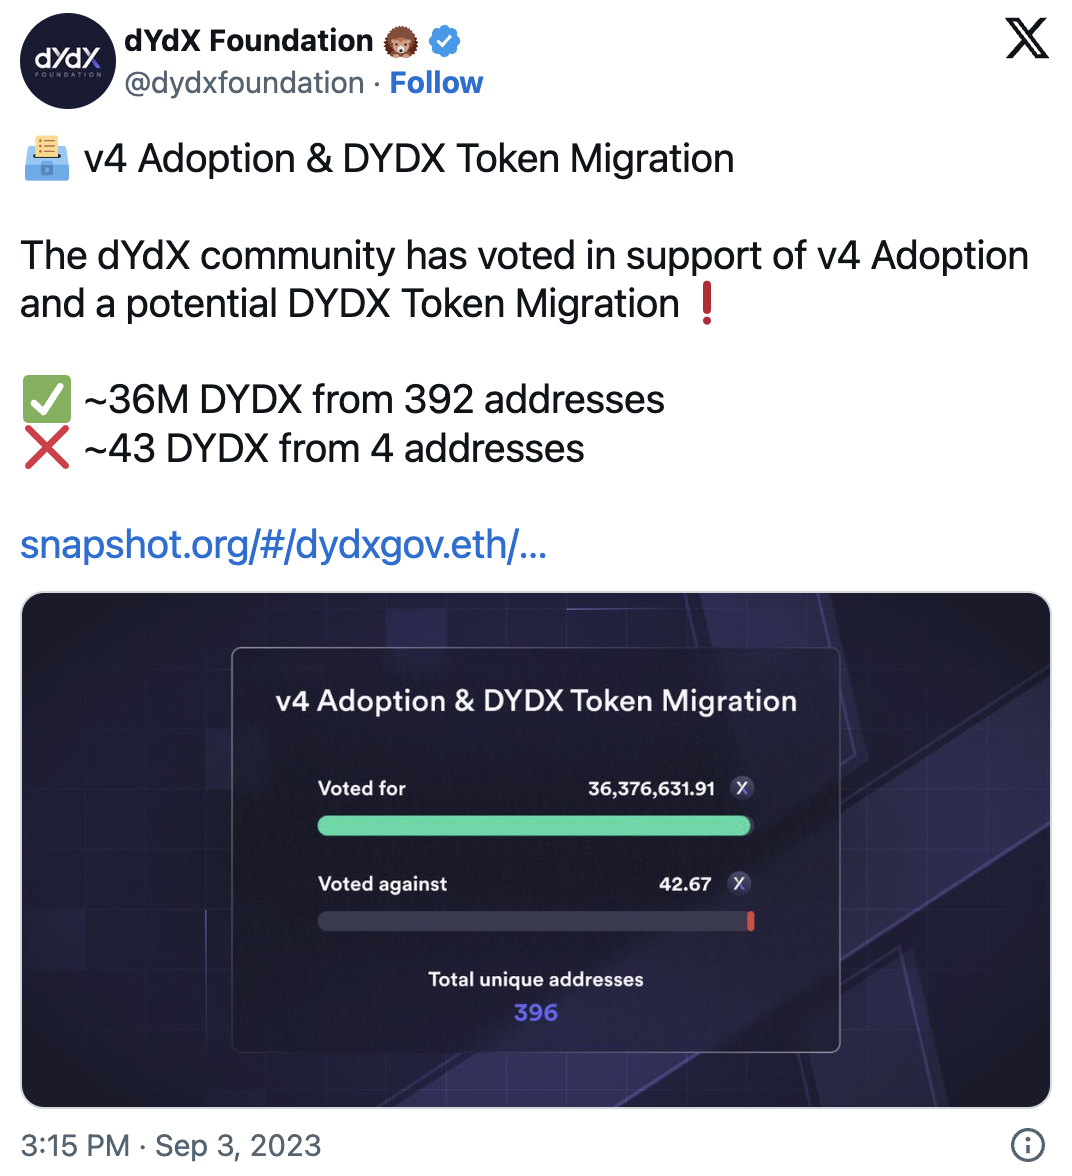
\includegraphics[width=\linewidth]{figs/migration_tweet.png}
            \caption{\bhref{https://twitter.com/dydxfoundation/status/1698414370512937319}{Tweet} from the dYdX Foundation on a successful vote to migrate the dYdX ecosystem from v3 to v4.}
            \label{fig:migration_tweet}
        \end{marginfigure}

    \subsection{Setting the L1 Token} \label{subsec:l1token}

        In the same governance proposal, Wintermute governance also proposed that the DYDX token should be the L1 token of dYdX Chain. In the authors' view, this was a natural choice for two main reasons: distribution and incentive alignment.

        A protocol, whether on Ethereum or its own Cosmos blockchain, seeks to involve the ``right people'' in its governance process. dYdX v3 already boasts a successful governance structure that rests on the distribution of ethDYDX token. dYdX Chain would ideally inherit this same distribution of ethDYDX to ensure its governance process is run by individuals that are already aligned with dYdX's interests, whether they are active users of the protocol, experienced delegates, or investors. As we will discuss in the following subsection, the process of bridging Ethereum-based ethDYDX to dYdX Chain aims to retain the existing distribution of governance tokens.

        We can roughly understand this incentive alignment in terms of financial stake in the success of the protocol. Ideally, a decision that harms the protocol will negatively affect the value of the governance token, whereas a good decision will increase value. This alignment fosters sound decision-making on behalf of the chain's governors (called stakers), and rests on the fact that the token's utility is tied to its decision-making and potentially interest-bearing role within the protocol's ecosystem. Recall that governance tokens on Cosmos chains are often interest-bearing because they receive rewards for being staked, such as a portion of  trading fees. 
        
        An example of a token with poorly-aligned incentives might be a stablecoin, such as USDC. If USDC were chosen as the protocol's governance token, then voters would be much less aligned with the protocol's goals. A short-term decision that damages the long-term prospects of the protocol but generates some revenue stream for governance could financially benefit stakers despite damaging the protocol. The value of staked USDC would not be at risk. Perhaps a less nefarious and more probable outcome is that USDC stakers would be less likely to actually vote on promising governance proposals for the protocol! Their only financial incentive is to earn interest from staking their USDC on dYdX Chain, they have no real exposure to the protocol's success outside of that yield, and they may simply procure yield elsewhere if dYdX Chain is unsuccessful. 
        
        Conversely, with DYDX as the chain's governance token there is a much stronger guarantee that the chain's stakers are motivated to properly govern the protocol and, in theory, increase the value of their holdings. They are incentivized to make decisions with the best, long-term interest of the protocol, since that is also in their financial best interest. There is also a much stronger guarantee that existing ethDYDX holders are familiar with the protocol. 

        Furthermore, electing any token other than DYDX token would disenfranchise the existing dYdX community, as those token holders would be stripped away of their hard-earned governance rights. 
        
    \subsection{The Ethereum to dYdX Chain Bridge} \label{subsec:tokentransition}

        \sidenotequote{In furtherance of its mission to support and promote the dYdX ecosystem by enabling communities, developers and decentralized governance, the dYdX Foundation has undertaken two activities in connection with a potential migration of the ethDYDX token from Ethereum to the dYdX Chain. First, it commissioned the development of an Ethereum smart contract that, if deployed, would enable a permissionless and autonomous one-way bridge for the ethDYDX token to be migrated from Ethereum to the dYdX Chain (as further described below). Second, it commissioned the development of source code that will be open-sourced such that others may use it to implement a user interface (also sometimes referred to as a “front-end”) to interact with such Ethereum Smart Contract.}{\bhref{https://dydx.foundation/blog/exploring-the-future-of-dydx}{Exploring the Future of dYdX}}Electing Ethereum-based ethDYDX token as the L1 token for dYdX Chain entails a significant technological and logistical challenge: how will ethDYDX token be bridged from Ethereum to dYdX Chain? 

        To support the ecosystem's migration from Ethereum to dYdX, the dYdX Foundation commissioned the development of a bridge from Ethereum to dYdX Chain, which was adopted by dYdX governance in a snapshot vote. We will describe this bridge in some detail so the reader understands what, exactly, is going on when they bridge their ethDYDX from Ethereum to dYdX Chain.

        Blockchain bridges essentially ensure that any bridged asset on the ``detination'' chain represents an equivalent claim on the original asset on the ``origin'' chain. A bridge connects an origin chain to a destination chain by locking up tokens in the origin chain and distributing an equivalent amount of tokens in the destination chain to some specified account. For example, a user might want to bridge ETH from Ethereum to Solana. The user sends 10 ETH to a bridge address on Ethereum, which then mints and disburses 10 ``bridged'' ETH on Solana to some specified account. Similarly, if a user sends 10 bridged ETH to that same bridge on Solana, they will receive 10 ETH on Ethereum. There is no actual ETH on Solana; bridged ETH is a brand new token that represents a claim on ETH on Ethereum.

        By that same principle the dYdX Chain bridge will receive ethDYDX on Ethereum, and validators on dYdX Chain will mint a new token on dYdX Chain, DYDX, to a specified account on dYdX Chain. The dYdX Chain bridge is itself a smart contract on Ethereum, implemented as a new ERC-20 token called wethDYDX. When a user interacts with the contract's \texttt{bridge} function, they simultaneously lock up their ethDYDX, mint and receive an equivalent amount in wethDYDX, and finally emit an event log in the contract stating that they have locked some amount of ethDYDX token. Validators on dYdX Chain listen to these event logs by connecting to an Ethereum RPC node. Once they acknowledge this new event log, they credit the specified address on dYdX Chain with an equivalent amount of DYDX tokens. For a more detailed explanation of the bridge, refer to the dYdX Foundation's \bhref{https://docs.dydx.community/dydx-token-migration/migration-of-dydx-from-ethereum-to-dydx-chain/wethdydx-smart-contract}{documentation}.

        Unlike most blockchain bridges, the bridge to dYdX Chain is a 1-way bridge. This means that once ethDYDX is sent to the bridge contract and locked, it cannot be retrieved. Instead, users receive wethDYDX, a new ERC-20 token. Although ethDYDX and wethDYDX might seem like the same token, their key difference is that ethDYDX can be bridged to dYdX Chain, wethDYDX cannot. By minting wethDYDX, the bridging contract allows bridgers to retain their governance rights on dYdX v3. Although the entire ecosystem is migrating to dYdX Chain, dYdX v3 must still be operated during the transition period, and potential governance proposals must continue to be submitted, voted on, and executed. To prevent dYdX v3 from becoming inoperable following the launch of dYdX v4, wethDYDX was introduced as a new candidate for dYdX v3 governance.

    \subsection{Upgrading v3 Governance}

        So far, all elements of the dYdX ecosystem's migration from Ethereum to Cosmos have been proposed by Wintermute governance. In the final step of their proposal, Wintermute also suggested that dYdX governance upgrades its \texttt{GovernanceStrategy} contract to account for wethDYDX when counting votes. For those unfamiliar, most governance solutions are implemented by a smart contract that tracks each voters' balance of the governance token, including any token that this user might have received or spent through delegation. dYdX v3's \texttt{GovernanceStrategy} contract was implemented as an upgradeable contract, meaning its logic can be modified to include new tokens when tallying voting power.

        The on-chain vote to upgrade the \texttt{GovernanceStrategy} contract has passed and been executed as of September 2023, and dYdX v3 now has two official governance tokens. Users bridging their ethDYDX to dYdX Chain may now participate in the governance process for both dYdX v3 on Ethereum, and dYdX v4 on dYdX Chain.\sidenote{Users should not interact with the wethDYDX bridge until the bridge's User Interface is released.}

    \subsection{Winding Down v3 Ecosystem Incentives}

        The migration from dYdX v3 to dYdX v4 also involves migrating Rewards programs. Since the ethDYDX supply is limited, the authors argue it is best spent on growing the v4 ecosystem. Xenophon Labs \bhref{https://dydx.forum/t/drc-bridging-the-community-and-rewards-treasuries/1258/3}{proposed} a gradual sunsetting of the v3 rewards programs according to the schedule on Figure \ref{fig:winddown}, starting on Epoch 30. Our primary reason for taking a gradual approach is to preserve the dYdX user experience. Both Trading and LP Rewards are meaningful parts of the user experience for takers and makers on dYdX v3. Many of these users must migrate their operations to dYdX Chain, which involves varying degrees of complexity: bridging, rewriting necessary code, learning about the new API for dYdX v4, etc.. This approach gives users a buffer period within which they can gradually shift their operations from v3 to v4.

        \begin{figure}[htp]
            \centering
            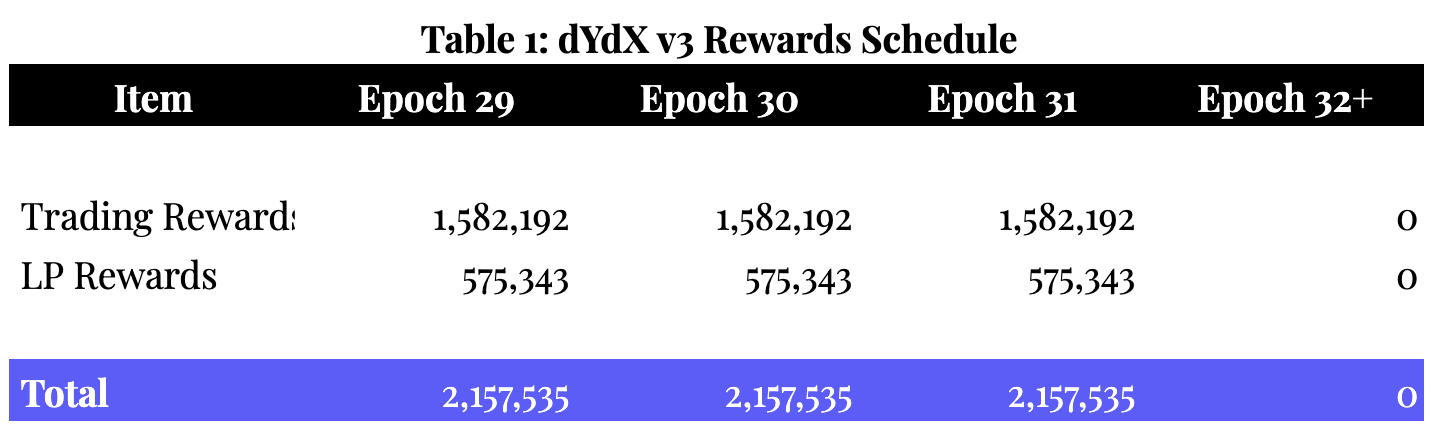
\includegraphics[width=\linewidth]{figs/reduction.png}
            \caption{Proposed dYdX v3 Rewards Emissions Schedule}
            \label{fig:winddown}
        \end{figure}
    
    \subsection{Bridging Community Resources}

        The dYdX community has control over two key financial resources, the \bhref{https://etherscan.io/address/0xe710ced57456d3a16152c32835b5fb4e72d9ea5b}{Community treasury} and the \bhref{https://etherscan.io/address/0x639192d54431f8c816368d3fb4107bc168d0e871}{Rewards treasury}. The Community Treasury is the primary financial resource the dYdX Community has to fund grants, new incentives programs, hackathons, etc.. In order for v4 governance to deploy this DYDX, it must first be bridged from Ethereum to dYdX Chain.  Otherwise, the dYdX community must rely on governance proposals on dYdX v3 to deploy capital, which poses a security risk if and when dYdX v3 is wound-down. The Rewards treasury is used to fund existing incentives programs, such as the Trading Rewards and LP Rewards programs that have been central to the growth of the dYdX ecosystem for the past two years. It must, like the Community Treasury, be migrated to dYdX Chain to fund the Chain's own Trading Rewards program.

        Bridging the community treasury is an incredibly delicate process involving the transaction of hundreds of millions of dollars worth of ethDYDX token. Xenophon Labs submitted a governance \bhref{https://dydx.forum/t/drc-bridging-the-community-and-rewards-treasuries/1258/3}{proposal} to begin this process, outlining 3 major steps for a successful transition:

        \begin{enumerate}
            \item Wind down the v3 ecosystem incentives.
            \item Bridge unvested ethDYDX tokens.
            \item Bridge vested ethDYDX tokens.
        \end{enumerate}

        We have described step (1) in the previous subsection. We now describe steps (2) and (3) of the treasury migration process.

        \subsubsection{Vested and Unvested ethDYDX}

            The treasury contracts both hold \textit{vested} ethDYDX, meaning ethDYDX that is available for transactions. They do not, however, hold the \textit{unvested} ethDYDX. Unvested ethDYDX, the vast majority of issued ethDYDX as of September 2023, sits in two vester smart contracts on Ethereum. The vesting occurs according to the schema in Fig. \ref{fig:govschema}, courtesy of the dYdX Foundation's \bhref{https://docs.dydx.community/dydx-governance/resources/technical-overview}{documentation}. 

            \begin{figure}[htp]
                \centering
                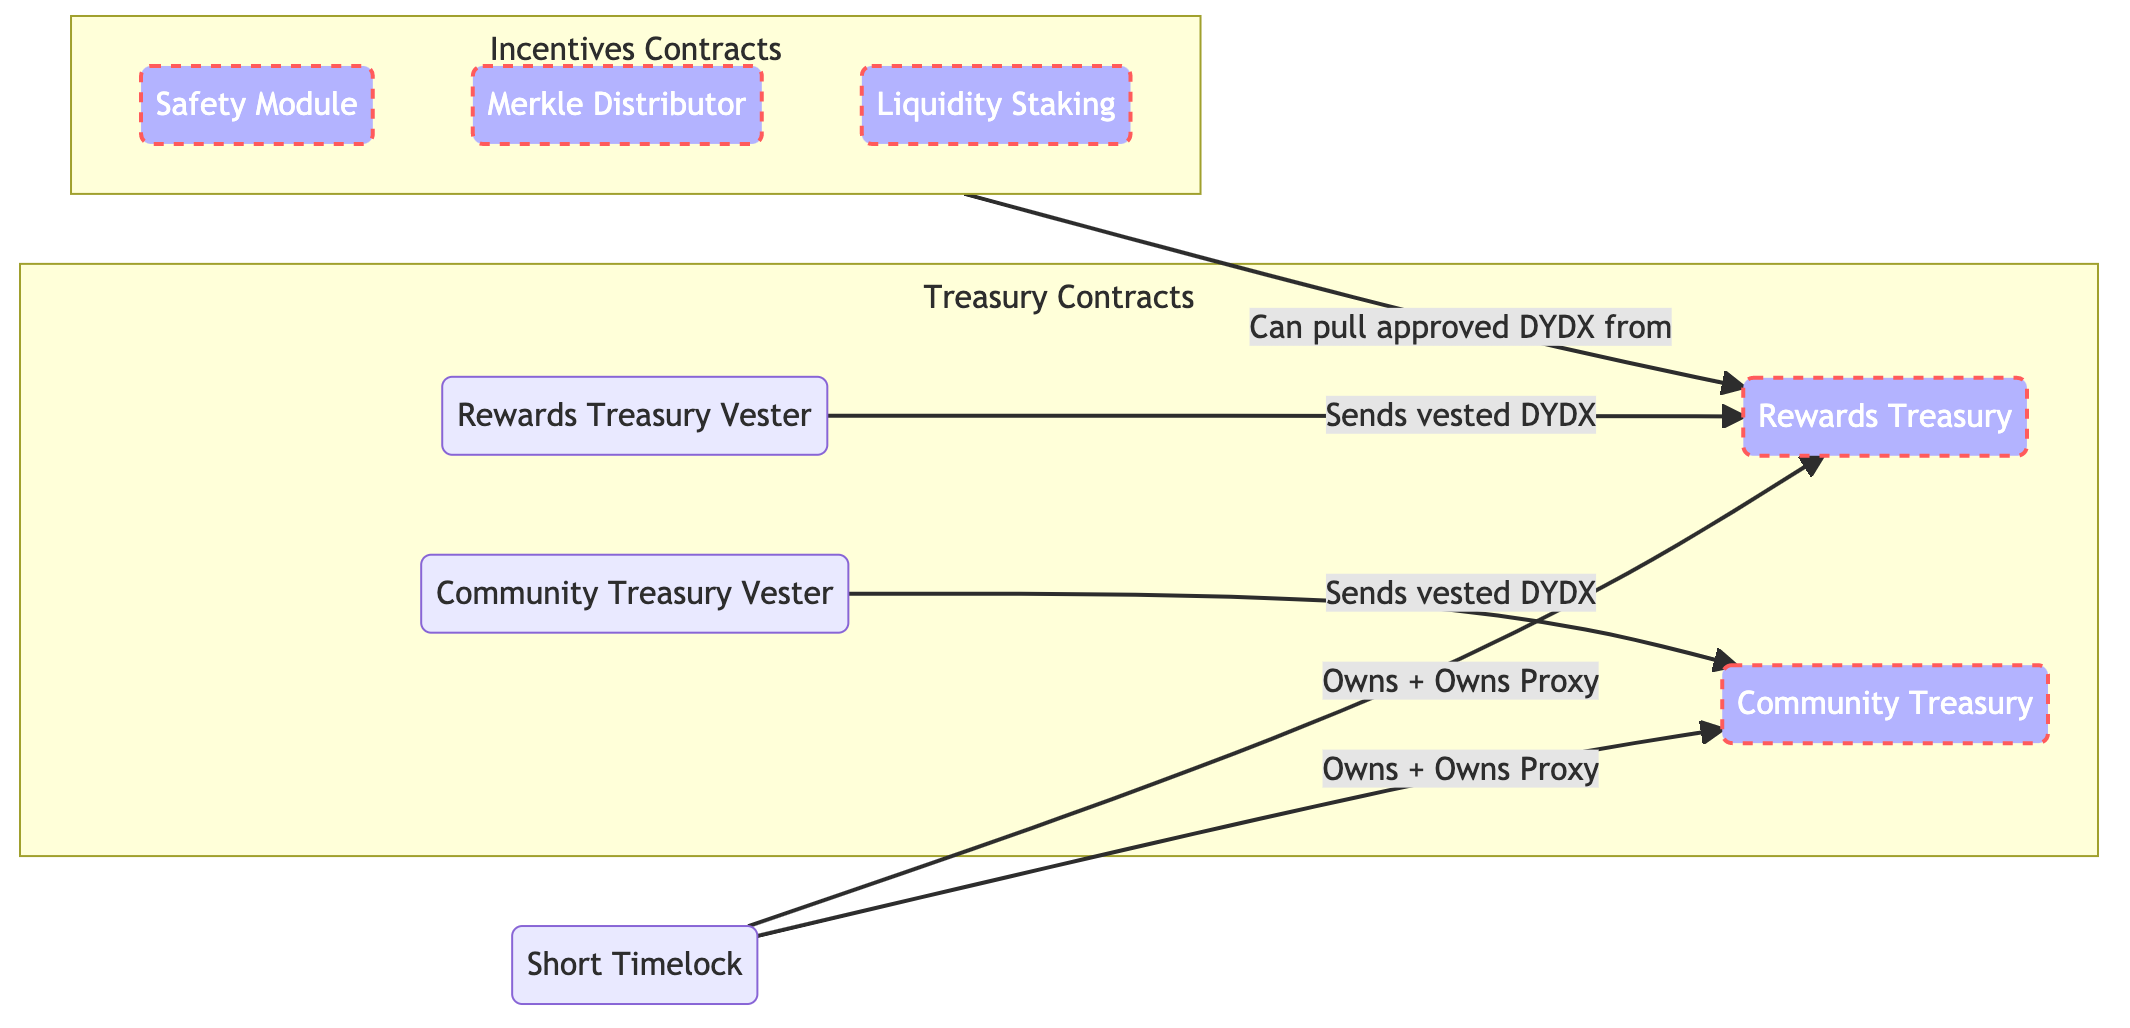
\includegraphics[width=\linewidth]{figs/schema.png}
                \caption{dYdX Treasury schema.}
                \label{fig:govschema}
            \end{figure}

            Vested ethDYDX can easily be bridged from Ethereum to dYdX Chain, since governance may submit transactions on behalf of each treasury. Since unvested ethDYDX is locked in the vester contracts, bridging unvested ethDYDX poses a greater challenge.

        \subsubsection{Upgrading the Treasury Contracts} \label{subsubsec:upgrade}          
        
            Both treasuries are implemented as upgradeable contracts controlled by a proxy administrator contract, in turn controlled by governance. In commissioning the creation of the Ethereum to dYdX Chain bridge, the dYdX Foundation also commissioned an upgraded version of the treasury contracts, appropriately named \texttt{TreasuryBridge}. The \texttt{TreasuryBridge} smart contract extends the existing treasury contracts in three important ways: (1) it claims all unvested ethDYDX on behalf of the current vesting recipient, (2) it then changes the vesting recipient, and (3) it implements a \texttt{bridgeTreasury} function.

            Suppose governance elected to change the vesting recipient of both vester contracts to a burner address, such as \texttt{0x00000}. Since the vesting recipient can only be changed by the current recipient, this would effectively burn all ethDYDX held within the vesting contracts. With all the unvested ethDYDX burnt, validators on dYdX Chain may then mint the equivalent amount of DYDX tokens on dYdX Chain, depositing them into vester contracts with identical vesting schedules. Effectively, the unvested ethDYDX has now been bridged to dYdX Chain, retaining the same vesting properties as it had on Ethereum. Crucially, this will require a successful governance proposal on dYdX Chain to credit the amount of ethDYDX burned on Ethereum to the appropriate vester accounts.

        \subsubsection{Bridging Vested ethDYDX}

            The community may choose to bridge the vested ethDYDX from the community and rewards treasuries into dYdX Chain using the \texttt{bridgeTreasury} function. The exact amount of ethDYDX to be bridged depends on the amount of ethDYDX vested at the time each contract was upgraded, and must account for the ethDYDX required to continue funding the v3 ecosystem incentives. Xenophon Labs has recently \bhref{https://dydx.forum/t/drc-bridging-the-community-and-rewards-treasuries/1258/3}{proposed} that $2,157,536$ ethDYDX should be kept in the Rewards Treasury to be distributed to rewards recipients on v3 for the remaining three epochs\sidenote{The exact amount needed to service the final epochs of rewards will likely exceed $2,157,536$ ethDYDX to account for any rewards that vest while the proposal is active.}. See the schema in Fig. \ref{fig:bridging} for a before-and-after illustration of the v3 and v4 treasury contracts.

            \begin{figure}[htp]
                \centering
                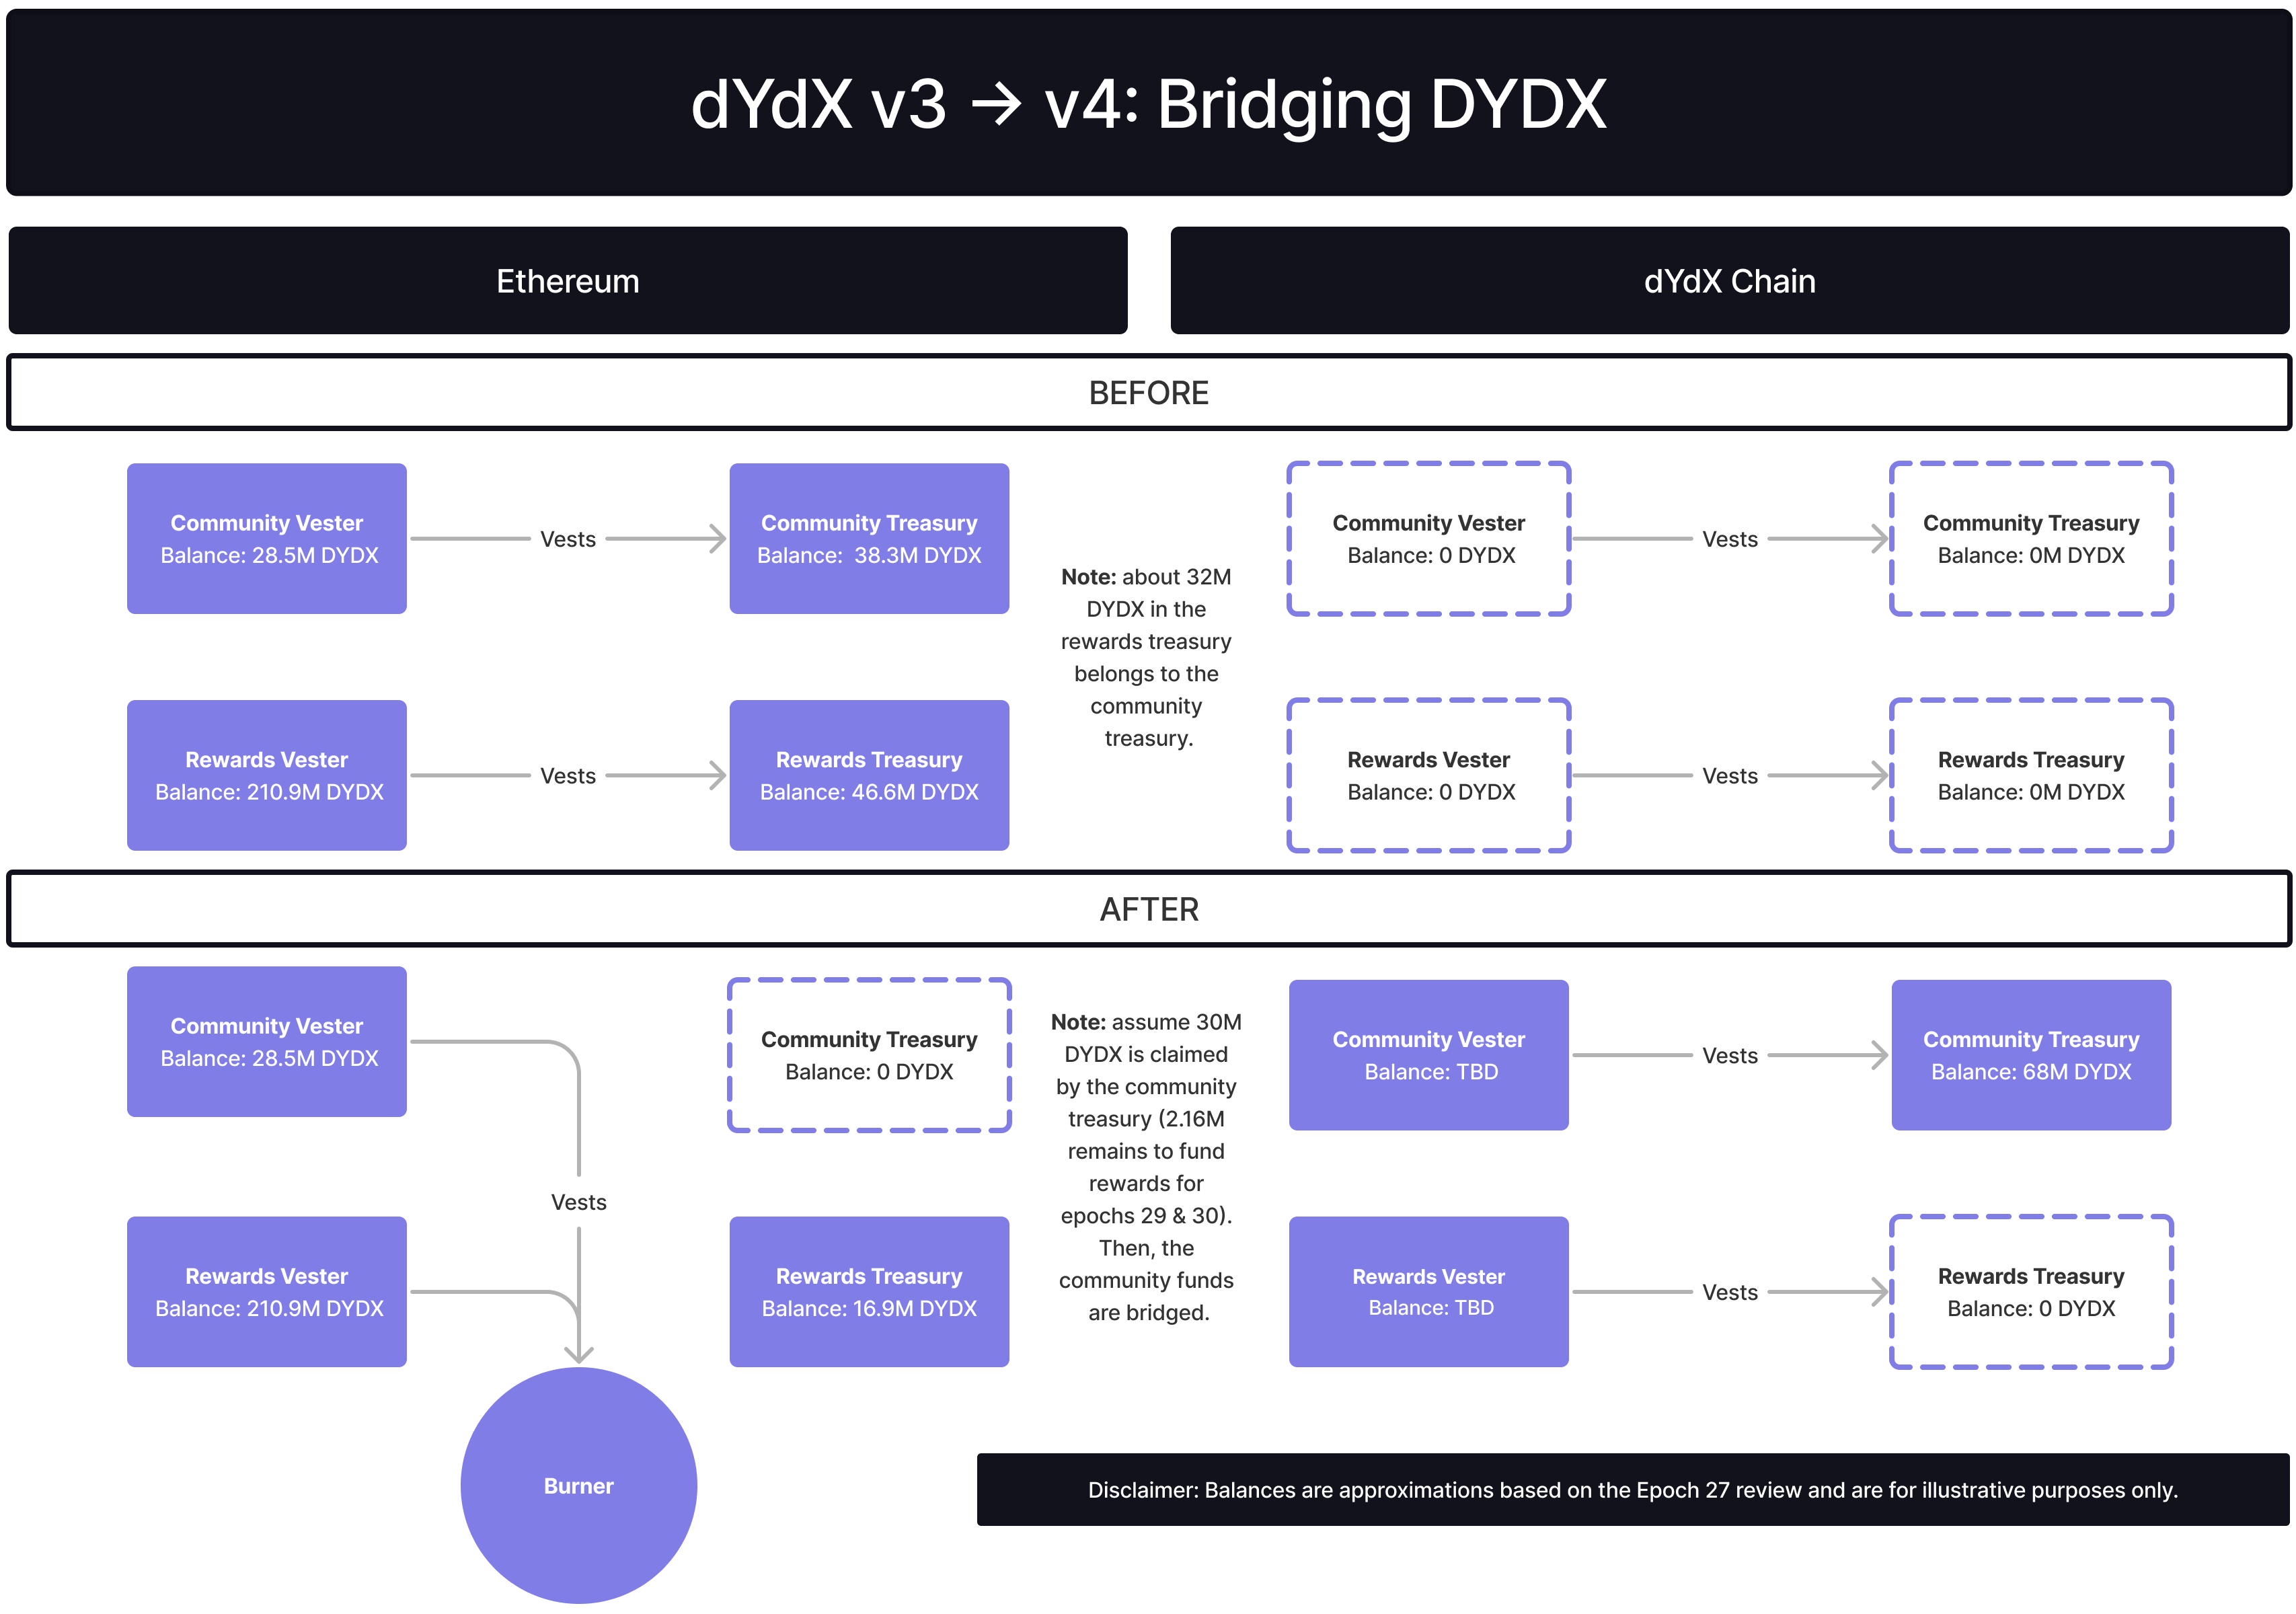
\includegraphics[width=\linewidth]{figs/Bridging.png}
                \caption{Before-and-after bridging the community and rewards treasuries to dYdX Chain.}
                \label{fig:bridging}
            \end{figure}

    \subsection{Liquidation Insurance Fund}

        Liquidations on dYdX v3 were performed by a liquidation engine, with the profit or loss from any given liquidation being counted against a liquidation insurance fund. Profitable liquidations increase the balance of the insurance fund, unprofitable liquidations decrease its balance. The current balance of the v3 insurance fund can be seen via the dYdX v3 API \bhref{https://api.dydx.exchange/v3/insurance-fund/balance}{here}. It hovers around \$20M.

        On dYdX v4, a similar insurance fund exists and requires funding. Accordingly, dYdX Chain governance may choose to fund the v4 insurance fund by performing an Over-the-Counter (OTC) transaction with a market maker on Cosmos, once community funds have been bridged to Cosmos. Although this proposal has not been submitted, the community may accomplish this by negotiating an OTC transaction with a trusted counterparty. This may be done permissionlessly on dYdX chain via governance proposals, or by trusting one of dYdX's subDAOs, such as the dYdX Operations Trust, to conduct the transaction.

        Once the insurance fund has been seeded with the requisite USDC, there is a stronger guarantee that the v4 liquidation engine will be able to close underwater positions despite potentially thin liquidity. For more information on liquidations and the insurance fund, see these posts from David Gogel at the dYdX Foundation: \bhref{https://help.dydx.exchange/en/articles/4797401-perpetual-contract-liquidations}{Perpetual Contract Liquidations} and \bhref{https://help.dydx.exchange/en/articles/4797358-contract-loss-mechanisms}{Contract Loss Mechanisms}.

    \subsection{Launch Incentives}

        \sidenotequote{Chaos Labs proposes a 6-month Launch Incentives Program to be deployed on V4. This program is designed to motivate the seamless migration of volume and users to V4.}{\bhref{https://dydx.forum/t/dydx-v4-launch-incentives-proposal/1075}{dYdX V4 Launch Incentives Proposal} by Chaos Labs}The cornerstone of DeFi user adoption has been user incentives programs. These have manifested as airdrops, liquidity mining, NFT giveaways, and other creative mechanisms for rewarding users for engaging with the protocol. To that end, a longtime contributor to the dYdX protocol, Chaos Labs, has proposed a new incentives program to bootstrap user adoption of dYdX Chain. 

        The Launch Incentives Program will be a novel kind of rewards program for dYdX. The program aims to incentivize two key behaviors on dYdX Chain: trading and deposits. To prevent sophisticated agents from being able to ``game'' or ``farm'' the program, Chaos Labs will not be disclosing the exact formula underpinning the rewards mechanism. Instead, the team will be periodically releasing the DYDX rewards earned by each account on dYdX Chain, with governance ultimately approving the disbursement of rewards through a governance vote. The more USDC you deposit on dYdX Chain, and the more you trade, the more rewards you will receive! 

        Up to \$20M USD (in DYDX) will be devoted to the program if current and future governance proposals are successful. The program will then leverage these funds to quickly acquire new users for the dYdX protocol and, hopefully, retain them.
        
    \subsection{The Migration So Far}

        We have overviewed the many components involved with migrating the dYdX ecosystem to dYdX Chain. This process has involved adopting a new governance token on dYdX v3, sunsetting existing incentives programs, launching new incentives programs on dYdX Chain, seeding an insurance fund, and more. Despite the complexity of the migration process, dYdX is successfully migrating its entire ecosystem to dYdX Chain while remaining committed to DYDX token holders and a decentralized governing process.